\documentclass{article}

\usepackage{fancyhdr}
\usepackage{extramarks}
\usepackage{amsmath}
\usepackage{amsthm}
\usepackage{amsfonts}
\usepackage{tikz}
\usepackage[plain]{algorithm}
\usepackage{algpseudocode}
\usepackage{graphicx}
\usepackage{gensymb}
\usepackage{calc}
\usepackage[framed,numbered,autolinebreaks,useliterate]{mcode}
\usepackage{listings}
\usepackage{empheq}
\usepackage{enumitem}
\usepackage{caption}

\graphicspath{{./images/}}

\usetikzlibrary{automata,positioning}

%
% Basic Document Settings
%

\topmargin=-0.45in
\evensidemargin=0in
\oddsidemargin=0in
\textwidth=6.5in
\textheight=9.0in
\headsep=0.25in

\linespread{1.1}

\pagestyle{fancy}
\lhead{\hmwkAuthorName}
\chead{\hmwkClass\ \hmwkTitle}
\rhead{\firstxmark}
\lfoot{\lastxmark}
\cfoot{\thepage}

\renewcommand\headrulewidth{0.4pt}
\renewcommand\footrulewidth{0.4pt}

\setlength\parindent{0pt}

%
% Create Problem Sections
%

\newcommand{\enterProblemHeader}[1]{
    \nobreak\extramarks{}{Problem {#1} continued on next page\ldots}\nobreak{}
    \nobreak\extramarks{{#1} (continued)}{{#1} continued on next page\ldots}\nobreak{}
}

\newcommand{\exitProblemHeader}[1]{
    \nobreak\extramarks{{#1} (continued)}{{#1} continued on next page\ldots}\nobreak{}
    % \stepcounter{#1}
    \nobreak\extramarks{{#1}}{}\nobreak{}
}

\setcounter{secnumdepth}{0}
\newcounter{partCounter}

\newcommand{\problemNumber}{0.0}

\newenvironment{homeworkProblem}[1][-1]{
    \renewcommand{\problemNumber}{{#1}}
    \section{\problemNumber}
    \setcounter{partCounter}{1}
    \enterProblemHeader{\problemNumber}
}{
    \exitProblemHeader{\problemNumber}
}

%
% Homework Details
%   - Title
%   - Class
%   - Author
%

\newcommand{\hmwkTitle}{Homework\ \#6}
\newcommand{\hmwkClass}{RBE 500}
\newcommand{\hmwkAuthorName}{\textbf{Arjan Gupta}}

%
% Title Page
%

\title{
    \vspace{2in}
    \textmd{\textbf{\hmwkClass\ \hmwkTitle}}\\
    \vspace{3in}
}

\author{\hmwkAuthorName}
\date{}

\renewcommand{\part}[1]{\textbf{\large Part \Alph{partCounter}}\stepcounter{partCounter}\\}

%
% Various Helper Commands
%

% Useful for algorithms
\newcommand{\alg}[1]{\textsc{\bfseries \footnotesize #1}}

% For derivatives
\newcommand{\deriv}[2]{\frac{\mathrm{d}}{\mathrm{d}#2} \left(#1\right)}

% For compact derivatives
\newcommand{\derivcomp}[2]{\frac{\mathrm{d}#1}{\mathrm{d}#2}}

% For partial derivatives
\newcommand{\pderiv}[2]{\frac{\partial}{\partial #2} \left(#1\right)}

% For compact partial derivatives
\newcommand{\pderivcomp}[2]{\frac{\partial #1}{\partial #2}}

% Integral dx
\newcommand{\dx}{\mathrm{d}x}

% Alias for the Solution section header
\newcommand{\solution}{\textbf{\large Solution}}

% Probability commands: Expectation, Variance, Covariance, Bias
\newcommand{\E}{\mathrm{E}}
\newcommand{\Var}{\mathrm{Var}}
\newcommand{\Cov}{\mathrm{Cov}}
\newcommand{\Bias}{\mathrm{Bias}}

\newlength\dlf% Define a new measure, dlf
\newcommand\alignedbox[2]{
% Argument #1 = before & if there were no box (lhs)
% Argument #2 = after & if there were no box (rhs)
&  % Alignment sign of the line
{
\settowidth\dlf{$\displaystyle #1$}  
    % The width of \dlf is the width of the lhs, with a displaystyle font
\addtolength\dlf{\fboxsep+\fboxrule}  
    % Add to it the distance to the box, and the width of the line of the box
\hspace{-\dlf}  
    % Move everything dlf units to the left, so that & #1 #2 is aligned under #1 & #2
\boxed{#1 #2}
    % Put a box around lhs and rhs
}
}

\begin{document}

\maketitle

\nobreak\extramarks{Question 1}{}\nobreak{}

\pagebreak

\begin{homeworkProblem}[Question 1]
    Consider the following robot joint model
    \[J\ddot{\theta}(t) + B\dot{\theta}(t) = u(t) + d(t)\]
    where $J$ is the inertia of the link, $B$ is the effective damping on the link, $\theta$ is the joint angle, $u$ is 
    the actuator torque (input), and $d$ is the disturbance acting on the system.
    \vspace{0.15in}\\
    First, assume that disturbance is zero and take \(J = 2\), \(B = 0.5\). Design a PD 
    controller such that the closed loop system is critically damped, and settling time is 2 second. Do 
    not do this by tuning the gains;  calculate  the  $K_p$  and  $K_d$  gains  using  natural  frequency  and 
    damping ratio.

    \subsection{Solution}
    Since $d(t) = 0$, \(J = 2\), \(B = 0.5\), we have

    \[2 \ddot{\theta}(t) + 0.5 \dot{\theta}(t) = u(t)\]

    Transform to Laplace domain,

    \begin{align*}
        2 \Theta(s) s^2 + 0.5 \Theta(s) s &= U(s)
    \end{align*}
    \begin{equation}
        \Theta(s) [2s^2 + 0.5s] = U(s)
    \end{equation}
    \begin{align*}
        \frac{\Theta(s)}{U(s)} = \frac{1}{2s^2 + 0.5s}
    \end{align*}

    Let our PD controller model be
    \[K_p e + K_d \dot{e} = u\]
    Transform to Laplace domain,
    \begin{align*}
        K_p E(s) + K_d E(s) s &= U(s)\\
        E(s) [K_p + K_d s] &= U(s)
    \end{align*}
    Therefore, the transfer function for the PD controller is
    \begin{equation}
        \frac{U(s)}{E(s)}=K_p + K_d s
    \end{equation}

    Now we can draw the block diagram, as shown below.

    \begin{figure}[h]
        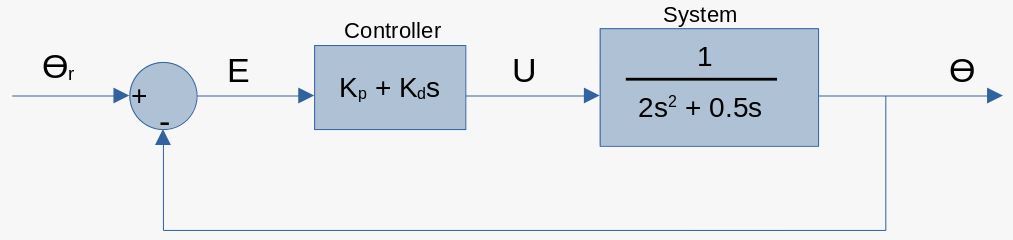
\includegraphics[scale=0.4]{q1-closed-loop-sys.png}
        \centering
    \end{figure}

    From the block diagram, we can see that
    \[E = \Theta_r - \Theta\]

    Using equation 2,

    \[\frac{U(s)}{K_p + K_d s} = \Theta_r - \Theta\]

    Furthermore, using equation 1,

    \begin{align*}
        \frac{\Theta(s) [2s^2 + 0.5s]}{K_p + K_d s} &= \Theta_r - \Theta\\
        \frac{\Theta[2s^2 + 0.5s]}{K_p + K_d s} + \Theta &= \Theta_r\\
        \Theta \left(\frac{2 s^2 + 0.5 s}{K_p + K_d s} + 1\right) &= \Theta\\
        \Theta\left(\frac{2 s^2 + 0.5 s + K_p + K_d s}{K_p + K_d s}\right) &= \Theta_r\\
    \end{align*}
    Therefore,
    \[
        \frac{\Theta}{\Theta_r}=\frac{K_p + K_d s}{2 s^2 + s(0.5 + K_d) + K_p}
    \]

    So our charateristic equation is,
    \begin{align*}
        2 s^2 + s(0.5 + K_d) + K_p = 0\\
        s^2 + s\frac{(0.5 + K_d)}{2} + \frac{K_p}{2} = 0
    \end{align*}

    The general form of the charateristic equation is
    \[s^2 + (2\xi\omega_n)s + {\omega_n}^2 = 0\]
    Where $\xi$ is the damping ratio and $\omega_n$ is the natural frequency.
    \vspace*{0.3in}\\
    Hence, we have,
    \begin{equation}
        {\omega_n}^2 = \frac{K_p}{2}
    \end{equation}
    and
    \begin{equation}
        2\xi\omega_n = \frac{(0.5 + K_d)}{2}
    \end{equation}

    Also, we know that the natural frequency and settling time $T_s$ are related by

    \[\xi\omega_n T_s = 4\]

    Since we are solving for a critically damped system, we set \(\xi = 1\). We also want settling time $T_s$ = 2 seconds.\\

    So, \begin{align*}
        \xi\omega_n T_s &= 4\\
        1 \cdot \omega_n \cdot 2 &= 4\\
        \omega_n &= 2
    \end{align*}

    Plugging this into equation 3, we have

    \begin{align*}
        {(2)}^2 &= \frac{K_p}{2}\\
        4 &= \frac{K_p}{2}\\
        \alignedbox{K_p}{=8}
    \end{align*}

    Also, plugging in values into equation 4, we have

    \begin{align*}
        2(1)(2) &= \frac{0.5 + K_d}{2}\\
        8 &= 0.5 + K_d\\
        \alignedbox{K_d}{=7.5}
    \end{align*}
\end{homeworkProblem}

\nobreak\extramarks{Question 2}{}\nobreak{}

\pagebreak

\begin{homeworkProblem}[Question 2]
    Follow steps in the assignment PDF file. Explain the process and be sure to include the plot to your report.

    \subsection{Solution}

    \begin{figure}[h]
        \centering
        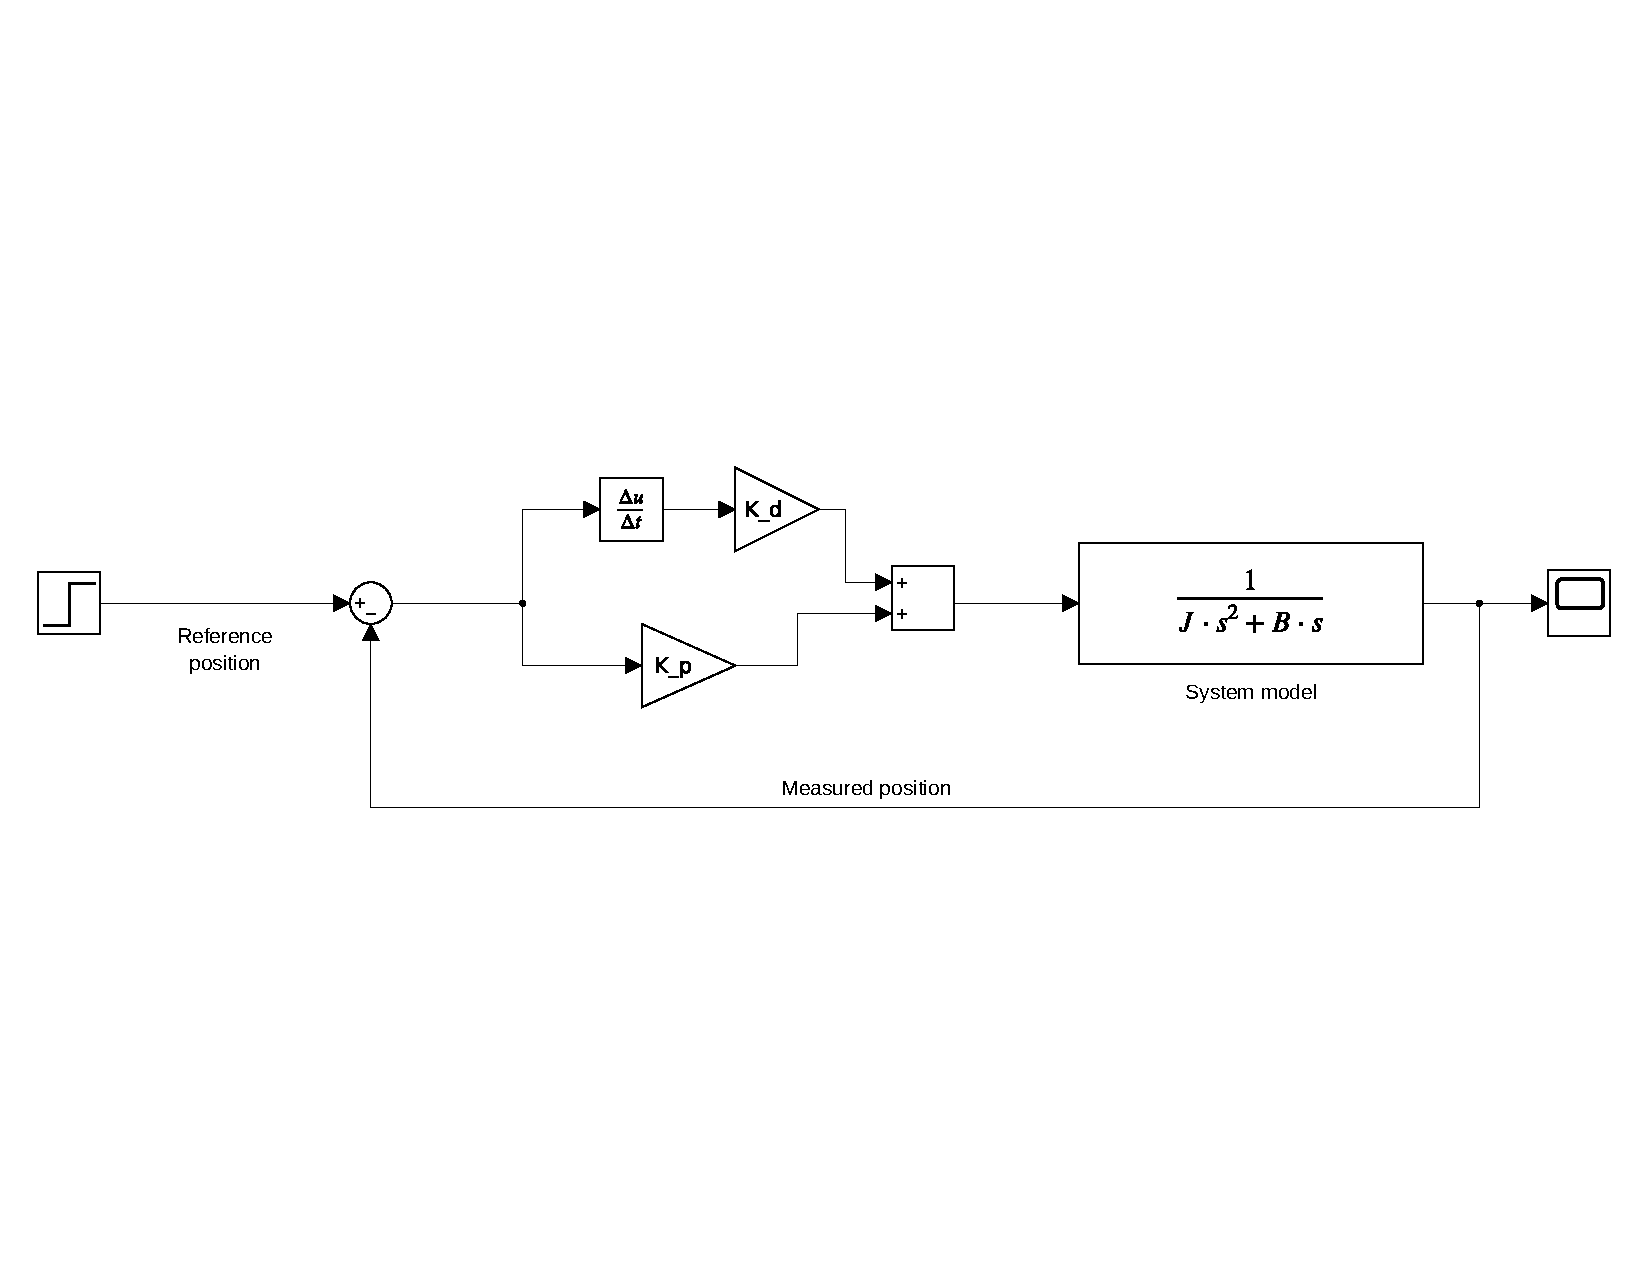
\includegraphics[scale=0.5]{hw6-q2-block-diagram.pdf}
        \vspace*{-5mm}
        \caption*{Block diagram for Question 2}
    \end{figure}

    After constructing the system model, here is the plot we obtained.

    \begin{figure}[h]
        \centering
        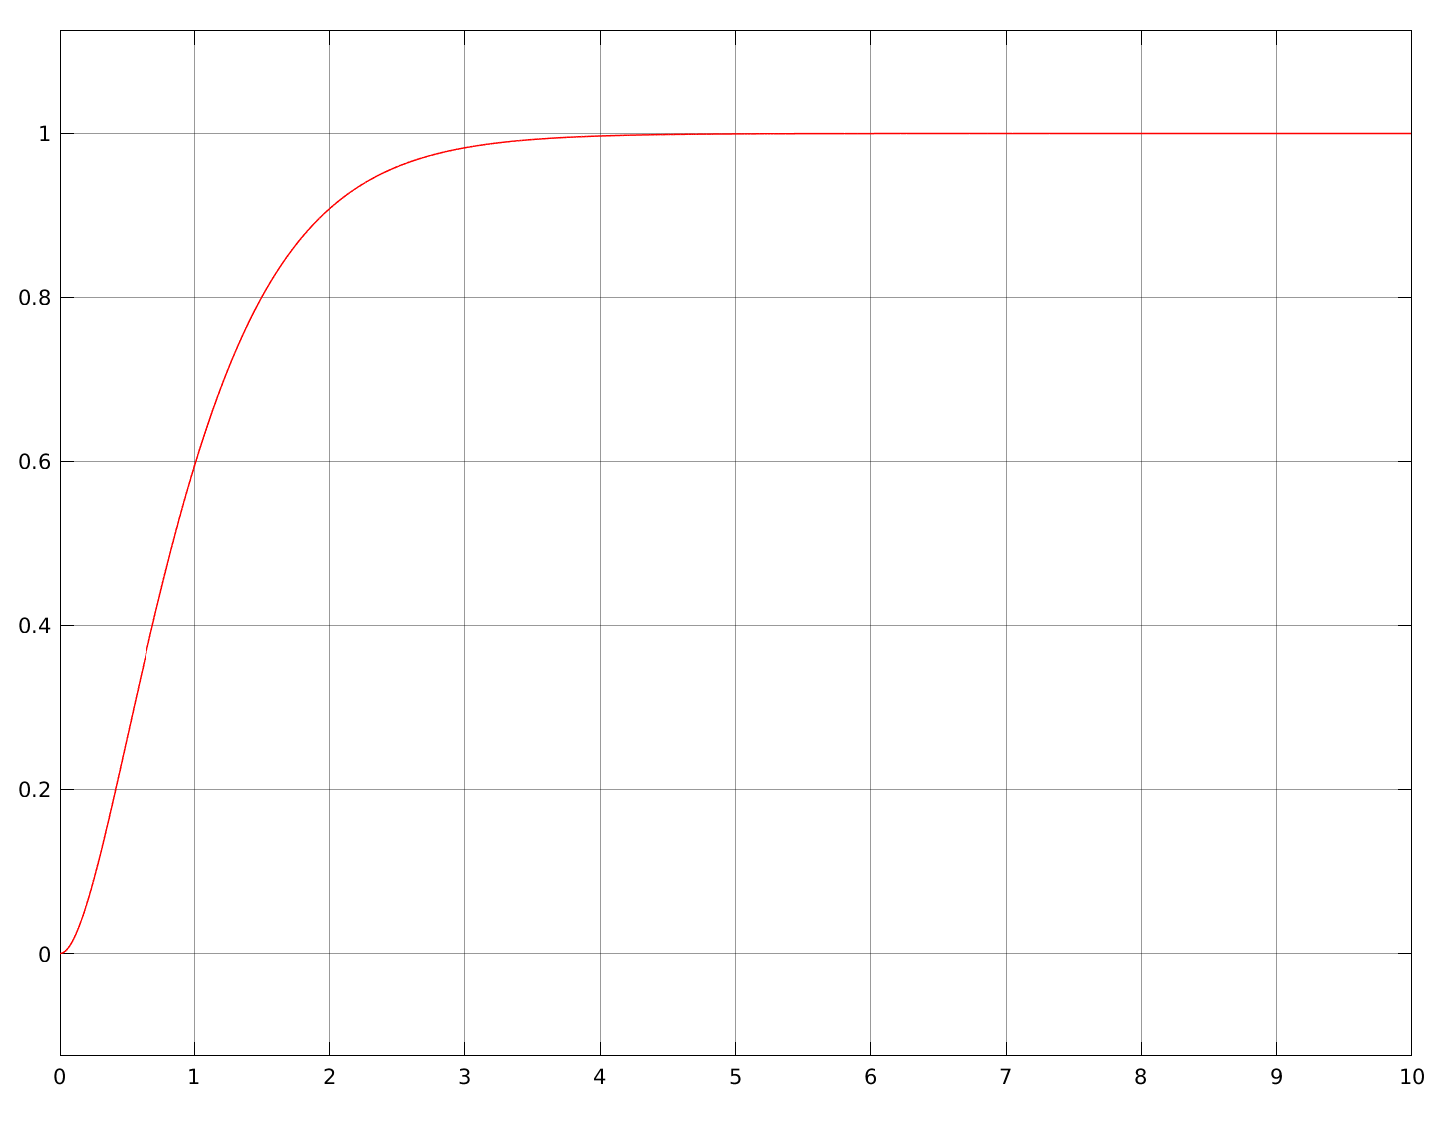
\includegraphics[scale=0.5]{hw6_q2_figure}
        \vspace*{-5mm}
        \caption*{Generated plot for Question 2}
    \end{figure}
\end{homeworkProblem}

\end{document}